\documentclass[11pt]{article}
\usepackage{listings}
\usepackage{graphicx}

\title{\textbf{COP 5615 - Distributed Operating Systems\\Project 2 - Failure Model}}
\author{Rahul Prabhu\\
		Sanil Sinai Borkar}
\date{\today}

\usepackage[parfill]{parskip}
\begin{document}

\maketitle

\section{Description}
The program was run with 2 additional parameters which indicated the failure type and percentage of the network that needs to go down. The following command was run at the sbt command prompt:
\begin{lstlisting}
$ run <numNodes> <numRequests> <failureType> <percentFailure>
\end{lstlisting}


There are 4 command-line arguments as given below:
\begin{enumerate}
\item \textbf{numNodes}: The number of nodes in the Chord P2P network. It is a positive integer value.
\item \textbf{numRequests}: The number of requests that each peer node has to make. Each such request will be made per second.
\item \textbf{failureType}: It could be any one of the following:
\begin{itemize}
\item {\it temporary} - The {\it percentFailure} number of nodes will ``sleep" for 1 second, and come back up.
\item {\it permanent} - The {\it percentFailure} number of nodes will permanently go down without informing any of the nodes in the network.
\item {\it leave}- The {\it percentFailure} number of nodes will inform the network before leaving.
\end{itemize}
\item \textbf{percentFailure}: Percent of the total number of nodes that need to fail. If the calculated number of nodes that need to fail was a real number, it was `floored' to the nearest integer.
\end{enumerate}

sbt will prompt to select the main class. Please select\\ \textit{edu.zeroday.chordbonus.ChordFailure}

In case of a permanent failure, the nodes go down without informing the network. This results in invalid entries in the finger tables of other nodes as well as invalid predecessor and successor pointers. This creates a problem during lookup and Chord may fail.

In case of nodes leaving the network, they inform the network about their leave wherein they update the finger tables of other nodes so that no invalid finger table entries exist. They also make sure to update the successor and predecessor pointers of their neighbors to the correct values before leaving. This ensures that lookups are performed correctly without failure of the network.

We tested the performance in each of the failure cases mentioned above. Temporary and permanent failures was achieved by maintaining the current `state' of an actor. It was initialized to the ``ALIVE" state, and was switched to ``DEAD" state to simulate its death. Once ``DEAD", in case of temporary failures, it came back up after a pre-defined time of 1 second. However, in case of permanent failures, it never came back up.

{\it Note: If failureType is entered as ``none", the program executes the normal implementation of Chord without failure models, which can be achieved by typing the following at the sbt command prompt:
\begin{lstlisting}
$ run <numNodes> <numRequests> none
\end{lstlisting}
}


\section{Chord}
With failures, chord took a lot more time and number of hops to deliver a message than the normal implementation. We used asynchronous messages to update the finger tables of other nodes. This adds more realistic behaviour to the failure model where the finger tables are not necessarily updated when a query comes through. Figure~\ref{chord_failure} shows the average number of hops taken to deliver messages in a network of 1000 nodes after {\it percentFailure} number of nodes failed for each type of failure.

\textit{For each combination of parameters, we ran the program a few times. The average of all the runs was then considered for our analyses and the graph plots.}
\begin{figure}[h]
    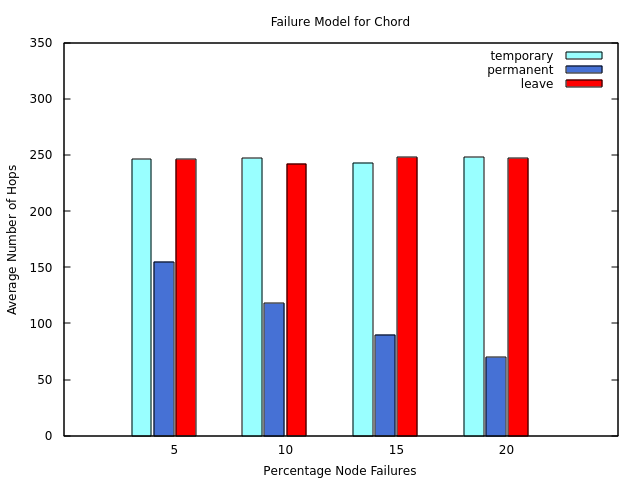
\includegraphics[scale=0.75]{images/failurechord.png}
    \caption{Chord run with various percentage of nodes failing}
    \label{chord_failure}
\end{figure}

\section{Observations}
\begin{enumerate}
\item {\bf Temporary Failures}\\
Once the node was up and running after its `temporary' downtime, Chord was able to do the lookup and the messages were delivered eventually. This happens because although the actor (node) goes to sleep temporarily, all the requests it receives are appended to its message queue but it does not process it. Once it wakes up, it starts processing these requests and delivers the messages. This leads to roughly the same number of hops as the normal implementation but takes more time.

\item {\bf Permanent Failures}\\
Since the nodes went down without informing, there was a portion of the network that contained stale entries in their finger tables plus some nodes had invalid predecessor and successor pointers. This virtually disconnected the network. As a result, lookup was not achieved, and some of the messages failed. The chord protocol expects the higher level applications using chord to handle such failures. Figure ~\ref{failure} shows the percentage of the total queries that were successful on different percentages of nodes failing.
\begin{figure}[h]
    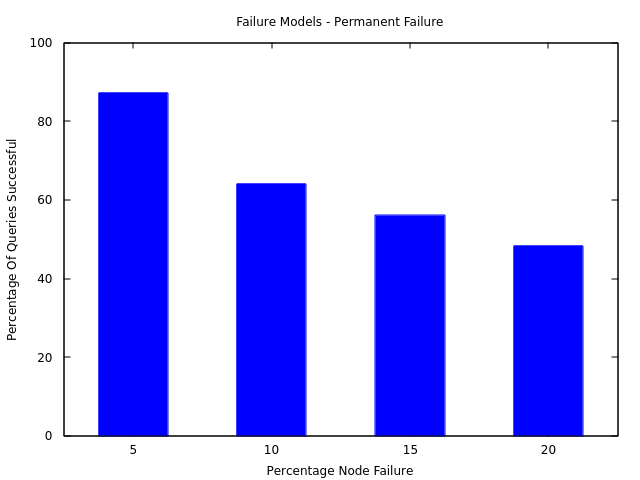
\includegraphics[scale=0.75]{images/permanentfailures.png}
    \caption{Chord run with various percentage of nodes permanently failing}
    \label{failure}
\end{figure}
\item {\bf Nodes Leaving the Network}\\
The nodes leaving the network inform the network so that all the nodes have up to date information. This is as if the nodes were never there in the network. Since the network remains stable with correct information, lookups take roughly the same amount of time and number of hops as in the normal implementation.
\end{enumerate}

\end{document}
